\section[Ring Modulators]{\textit{Ring Modulators}}
\sectionmark{\textit{Ring Modulators}}
\label{sec:ring_modulators}

El modulador en anillo o \textit{ring modulator}, fue inventado por Frank A. Cowan en 1934 con una finalidad práctica en el campo de la telefonía. Su nombre procede de la forma del circuito analógico, la de un \textit{anillo} de diodos. El producto de la modulación en anillo de dos señales cualesquiera es una señal compuesta por la suma y la diferencia de las frecuencias presentes en aquellas. La aproximación más sencilla al procedimiento analógico de este efecto es el de la multiplicación de ambas señales de entrada en el dominio del tiempo. La diferencia con la \textit{amplitud modulada} es que las frecuencias de las señales de entrada no están presentes en su producto. 

Este procesado de la señal adquiere interés sonoro cuando una de las dos señales de entrada --típicamente llamada <<portadora>>\footnote{Ya que el \textit{output} del \textit{ring modulator} equivale a la multiplicación de dos señales, ambas son equivalentes en términos matemáticos debido a la propiedad conmutativa de la multiplicación. Los términos <<señal moduladora>> y <<señal portadora>> son intercambiables.}-- tiene una forma sinusoidal u otra simple. 

\begin{figure}
	\centering
	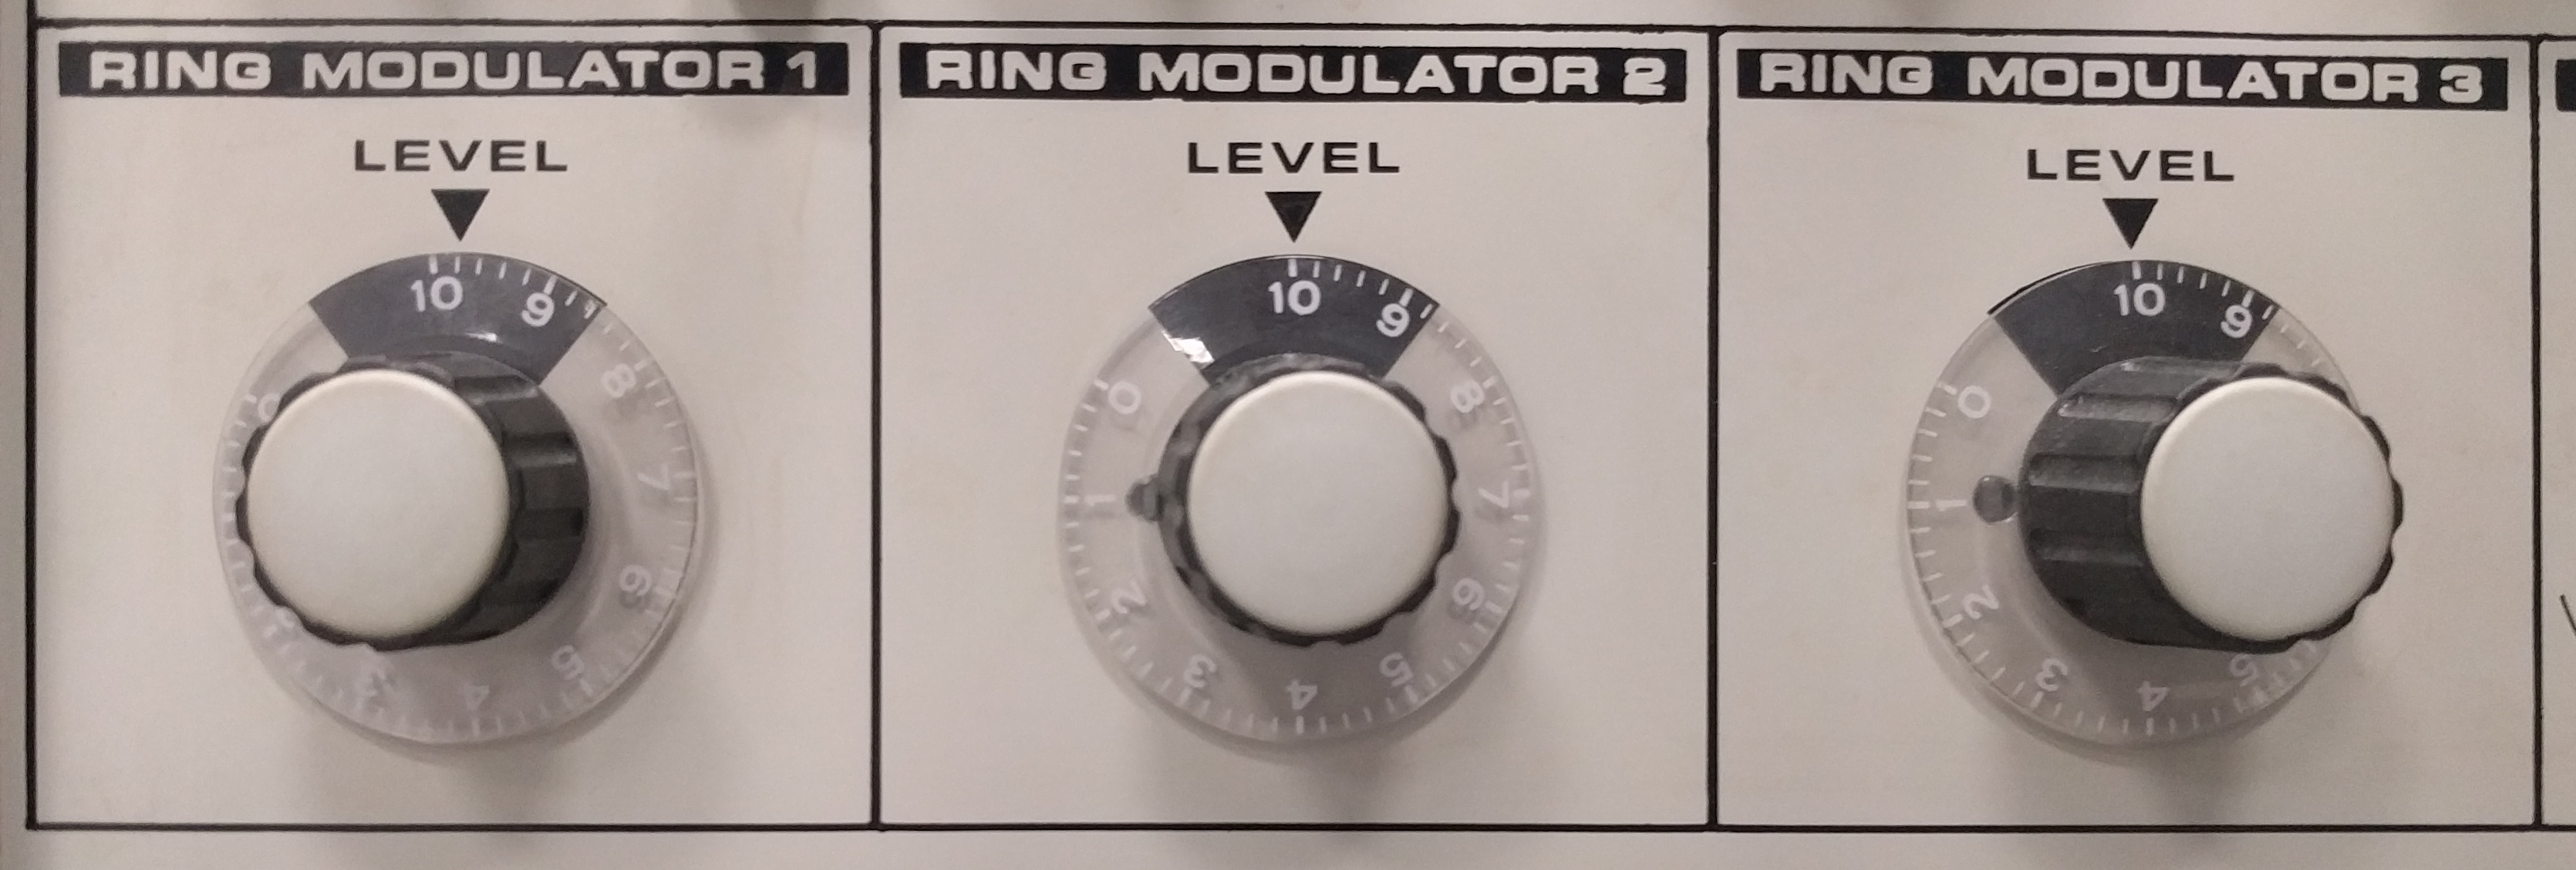
\includegraphics[width=0.7\textwidth]{images/ring_modulators}
	\caption[\textit{Ring Modulators}]{Los tres moduladores en anillo del Synthi 100 del GME.}
	\label{fig:ring_modulators}
\end{figure}

El Synthi 100 tiene 3 moduladores en anillo, y su único mando de control es un dial de ganancia (\textit{Level}). Sus entradas y salidas son exclusivamente de audio, aunque, gracias a la posibilidad de comunicar \textit{busses} con entradas de audio hacia salidas de voltaje (Ver \ref{sec:output_channels}), la salida de \textit{Ring Modulator} es susceptible --como el salidas de cualquier módulo-- de ser utilizada como un voltaje de control.

\appName~ implementa una simple multiplicación de las dos señales de entrada, con lo que se trata de uno de los módulos de menor coste de computación de toda la aplicación, al no intervenir ningún \textit{UGen} de procesado de señal.